% File clic2021.tex
% May 2021

%% Based on the style files for CLiC-IT-2019

\documentclass[12pt]{article}
\usepackage[a4paper]{geometry} 
\usepackage{graphicx} % Required for inserting images
\usepackage{clic2023} % imports CLiC-it 2023 layout style
\usepackage{times} % font 
\usepackage{xurl} % splits URL in multiple lines
\usepackage[italian,english]{babel}
\usepackage{latexsym} 
%\pagenumbering{gobble} % does not display page numbering
\usepackage{xcolor}
\usepackage[square,numbers]{natbib}
\bibliographystyle{unsrtnat}


\setlength\titlebox{5cm}

% You can expand the titlebox if you need extra space
% to show all the authors. Please do not make the titlebox smaller than 5cm (the original size); we will check this in the camera-ready version and ask you to change it back.


\title{Ethical Issues of Using Blockchain and NFT Technology for Digital Trades}

\author{\textbf{Sama Samrin, ID: 1191609, Computer Science Department, Lakehead University} 
}

\date{}

\begin{document}
\maketitle
\begin{abstract}
{\color{blue}\textbf{ Built on blockchain technology, Non-fungible Tokens (NFTs) have risen in popularity since 2021 as a unique medium of purchasing or trading digital art using cryptocurrencies like Ethereum. Although it provides a viable alternative for modern artists to have a digital ownership of their authentic creations and earn from them via features like royalty agreements, it simultaneously impacts the environment adversely and operates on problematic regulations. The relevant issues cover a wide spectrum including stolen art, untested smart contracts, influencer scams and more. In this study, we will take a deeper look at how the NFT technology and its regulatory vulnerabilities have been exploited by malicious individuals to implement fraudulent schemes, money laundering and similar criminal activities.}  }

\textbf{\emph{Index Terms-} Ethics, Blockchain, NFTs, Ethereum.}
\end{abstract}


\section{Introduction}

When social media platforms began their journey in late-to-mid 2000s, another revolutionary technology was brewing side by side. The mysterious figure called Satoshi Nakamoto built the first ever blockchain network and introduced it in 2008 \cite{nakamoto2008bitcoin}. His paper also presented the earliest cryptocurrency called Bitcoin and described how each component of this novel technology functions to provide a decentralized system for financial transactions without the involvement of financial institutions. 


{\color{blue}
This blockchain technology allows peer-to-peer monetary transactions between participants who exist on the same blockchain network. These transactions are then approved by consensus and recorded on a digital decentralized ledger, which is accessible from each participant’s device. Each party gets two kinds of digital keys - public (which can be shared with anyone) and private (which must be kept secret).} The later sections delve deeper into the details of blockchain technology. This entire blockchain architecture and technology is the backbone and source of power for several rapidly growing fields today including artificial intelligence, big data \cite{modanimethodological} and NFTs.

{\color{blue}
NFT or Non-fungible Token is a unique cryptographic representation of ownership for digital, virtual and occasionally physical assets. Professor Michael Dowling \cite{DOWLING2022102097} defines NFTs as “tradeable rights to digital assets (images, music, videos, virtual creations) where ownership is recorded in smart contracts on a blockchain”. Even though it gained popularity in this decade, the first ever NFT was a video clip tokenized by Kevin McKoy in 2014 \cite{9803425}.

Since then, both NFT space and cryptocurrency universe have undergone many changes and achieved numerous milestones.  On one hand, NFT is considered to be a strong solution for patent protection \cite{barakat2022use}, digital copyright issues \cite{Rafli_2022} and low profit share of artists \cite{Chainalysis}. On the other hand, with more sets of eyes on such activities, there has also been an increase in malicious intruders finding loopholes in blockchain technology to satisfy their greed. Determining the causes, types and solutions to these issues is extremely important for ensuring  the safety of current and future groups of artists, traders and crypto experts.}

\section{Literature Review}

Although Satoshi Nakamoto’s paper is widely regarded as the earliest concept of blockchain, its primary skeleton of connected blocks with cryptographic chains is actually an idea from the 1990s. In the paper titled “How to time-stamp a digital document” published in the Journal of Cryptology in 1991 \cite{modanimethodological}, authors Stuart Haber and W Scott Stornetta described using hash functions and digital signatures to convert analog files into their digital format. It presents a method where the Trusted Time Stamping (TTS) takes the calculated hash and the digital signature of a document to send it to another user. 

Based on this method, Nakamoto developed the modern blockchain technology and a peer-to-peer electronic cash system in 2008 \cite{nakamoto2008bitcoin} that does not hand over its power to a central authority. This decentralized infrastructure would facilitate an impregnable method for online transactions using digital signatures, encryption and proof of work based on hash functions. It would eliminate the need for a third party or a financial institution to verify and secure each transaction. The first successful and most popular digital currency Bitcoin came into the picture which utilized the blockchain technology. 

The popularity of blockchain skyrocketed in late 2010s as a cutting-edge technology to improve data security, storage and speedy transfer between individuals across the planet. Even though it was launched with Bitcoin (BTC), the evolution of this technology climbed a level higher using the other popular cryptocurrency named Ethereum (ETH) \cite{ante2022non}. Ethereum’s token standard \cite{wang2021non}, more specifically ERC-20 \cite{ali2021introduction}, is what the concept of NFT comes from. Besides, most NFT marketplaces like OpenSea and Rarible uses Ethereum as the primary currency for trading and purchase purposes \cite{9869497}. 

These groundbreaking platforms of selling and trading digital assets has gone from generating monthly sales worth over 8 million USD in 2021 to over 4 billion USD in 2022 \cite{mekacher2022heterogeneous}. However, a number of these sales had been conducted with fraudulent behavior and false promises made by scammers \cite{9755212}. Malicious individuals at various hierarchy levels have taken advantage of the hype around NFTs and the lack of relevant knowledge among people to get away with their dishonest strategies. For instance, the product head of OpenSea, Nate Chastain admitted to being part of an insider trading scam in September 2021 \cite{scharfman2023non}. Combining its social media traction, lack of public knowledge, and the vulnerabilities of its underlying technologies, cybercriminals and fraudsters have scammed unsuspecting users by promoting fraudulent projects online. The social media platform Twitter alone has been the brewing ground for numerous scamming promotions like this. A study revealed that more than 36\% of the NFT projects promoted within two months here were fraudulent \cite{roy2023demystifying}. 

Additionally, NFTs are also being used for operating illegal activities like wash trading \cite{vonwachter2022nft} and money laundering \cite{kafteranis2022art}. The promise of a future dependent on metaverse intensifies the public inclination to gamble with their money for a miraculous financial win. After e-commerce and f-commerce, metaverse commerce is expected to be the next big trend where one can trade digital assets and properties in the virtual world \cite{lee2021all}.

\section{Fundamentals of NFT Technology}

\subsection{Blockchain Technology}
Blockchain is named after its structure whose base consists of data blocks chained to each other \cite{ali2021introduction}. In its earliest days, it was considered to be a revolutionary foolproof medium for instantaneous financial transactions between accounts on a decentralized peer-to-peer (P2P) network, because of its immutable ledgers \cite{abid2021uses}. The immutability represents how each transaction data is recorded on its interconnected blocks using cryptographic hash functions and therefore such information cannot be altered in a feasible manner \cite{rahardja2021immutability}. 

\begin{figure}
    \centering
    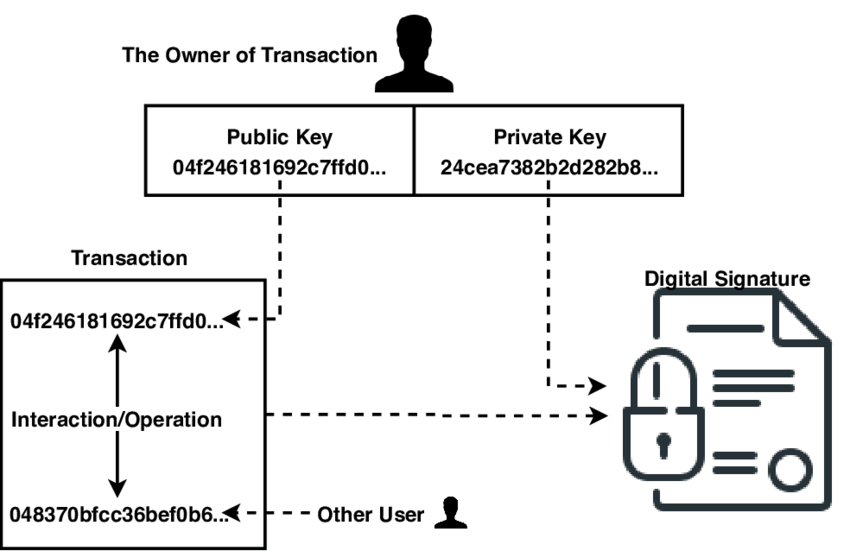
\includegraphics[width=8cm]{Simplified-scheme-of-a-blockchain-transaction.png}
    \caption{Simplified Blockchain Transaction \cite{aydar2019private}}
    \label{fig:block}
\end{figure}

A blockchain address is a unique specific sequence of alphanumeric characters consisting of a private key and a public key. It functions similar to a bank account number than can identify a unique user. The owner of a blockchain address has to share his public key to conduct a transaction successfully while his private key will remain hidden from other users. In the case of NFT, these users are basically owners of active blockchain or cryptocurrency wallets.

Owners of a cryptocurrency perform each digital transaction on the blockchain by adding data of the previous transaction, his private key and the receiver’s public key to the end of his coin. After sending it with the right digital signature, the receiver verifies this signature and validates the new ownership. 

A central authority called mint generates new coins, authenticates data, and prevents double-spending in each transaction. The Proof of Work (PoW) protocol \cite{xiao2020modeling} functions as the most prominent consensus mechanism adopted by the network members (or nodes) to prevent unauthorized database access and suspicious transactions. According to Nakamoto, this mechanism promotes data security “as long as honest nodes collectively control more CPU power than any cooperating group of attacker nodes”. That is because the extent of control or authority held by each member is proportional to the amount of computing power they offer for crypto mining \cite{xiao2020modeling}.

\subsection{Smart Contract}
Smart contract is originally the brainchild of Nick Szabo who first proposed the concept in 1996 \cite{szabo1996smart}. These {\color{blue} digital agreements called smart contracts are basically computer programs embedded within the blockchain. Kai Peng et al \cite{9409120} define it as “a decentralized program with a set of self-enforcing agreements on the blockchain”.} It is programmed to run automatically during an agreement when the preset conditions are triggered between the buyer and the seller \cite{chen2019secure}. This combination of code (event or function) and data (state) is typically implemented within the Ethereum blockchain \cite{ali2021introduction} to enforce its rules, such as ensuring that the user has the right cryptocurrency and the security protocols like lockbox are in place.

\begin{figure}
    \centering
    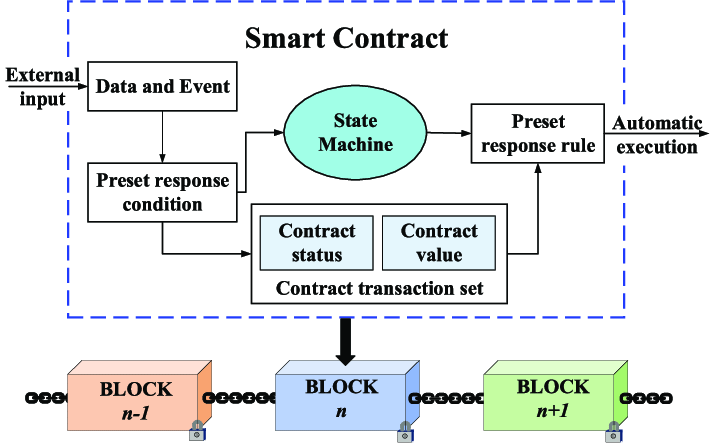
\includegraphics[width=8cm]{Smart-contract-model-based-on-energy-blockchain.png}
    \caption{Smart contract model in a blockchain \cite{chen2019secure}}
    \label{fig:smart}
\end{figure}

{\color{blue} Unlike regular contracts, a smart contract is immutable and distributed, i.e. no one can change it after creation and everyone on the network needs to validate it.} Once it has started, none of the participants can pause or stop it. The applications developed with a smart contract in the back-end, running on decentralized platforms like Ethereum, are called decentralized apps or DApps \cite{mishra2020implementation}. Smart contracts are indispensable to most NFT ecosystems since they safeguard the order-sensitive executions required in blockchains.


\subsection{NFT}
{\color{blue} The term ‘fungible’ is typically used to represent inherently valuable items that can be exchanged with other items of the same category. For instance, common money or notes of the same currency is a fungible item, because it has intrinsic value and you can exchange a 20 CAD note for two 10 CAD notes. Similarly, cryptocurrencies residing on the same blockchain are interchangeable and they can be exchanged for fiat currencies as well (such as GBP, Euro and Chinese Yuan) \cite{UMAR2021121025}.


Unlike them, NFTs are non-fungible tokens because they are not interchangeable even when they are on the same blockchain \cite{Investopedia}. They can be traded for other NFTs but not substituted.}

Originating from Ethereum token standards, specifically EIP-721 \cite{cabot2022improving} and EIP-1155 \cite{chen2022toward}, the NFT technology is equipped with the ability to distinguish between tokens \cite{wang2021non}. It facilitates transferring rights to digital assets like audio, video, image and other collectibles with the help of cryptocurrency wallets and blockchain infrastructure. The markets of NFTs and cryptocurrencies are interdependent \cite{ante2022non} since a user must have a crypto wallet in order to create, sell, or trade NFTs.

{\color{blue} New NFTs are generated through the minting process where their unique information is recorded on a newly created block of the blockchain and then verified by a validator. To ensure the safety of transactions and ownership transfers, every NFT needs to follow standards like ERC-721 or ERC-1155 \cite{9803425}. Minting also allows the creator to set the price, rules and royalties for the NFT \cite{10.1145/3474355} in the corresponding encoded smart contract.}

\section{The Promises of NFT Technology}
The whole concept of NFTs gained momentum because of the frequent issues it showed the potential to resolve. One of the most prominent promises it had was providing digital artists or creators a feasible way to protect their original creations from plagiarism. It is very easy to copy and save an image, audio, video, document or any other file one finds on the internet. Utilizing the uniqueness of NFT properties, the original creators can prevent others from using their authentic creations for commercial purposes. They can maintain their ownership of the original material and only transfer this ownership to someone else in exchange for an adequate price. This system makes sure that the digital content creators are getting a proper compensation for the time and labor they invested into that project.

This kind of digital art also has a promising future in virtual spaces like metaverse. It has been rising in popularity among users who want to flaunt their artistic taste to their virtual friends. Some would also like to use such NFTs to attract new buyers and sell them as digital collectibles via bidding. For instance, the traditional auctioning platform Sotheby’s held an online auction in June 2021 \cite{lambert2021beyond} where it sold a number of early raw NFT artworks from four continents in a remarkable collection named Natively Digital. Such activities open up more doors for digital creators to earn a living and inspire them further to continue in their creative endeavors.

Moreover, its backbone of blockchain technology was meant to assure people about how illegal sales of NFTs can be easily detected via its publicly accessible records on the ledger. However, the reality presented with its failure regarding data security, unauthorized access prevention and more such struggles discussed in the upcoming section. 

\section{Ethical Challenges of NFT Trades}
{\color{blue} NFT primarily garnered popularity in the public eye in mid-2021. According to the annual Crypto Crime Report published by Chainalysis \cite{Chainalysis}, the amount of cryptocurrency sent to Ethereum-based smart contracts increased from \$106 million in 2020 to at least \$44.2 billion in 2021 [Figure 3].

\begin{figure}[ht]
\centering
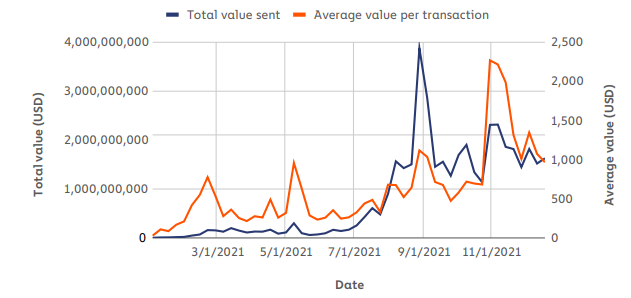
\includegraphics[width=8cm]{fig}
\caption{Weekly total cryptocurrency value and average value per transaction sent to NFT platforms throughout 2021, Chainalysis Cyber Crime Report 2022}
\end{figure}

This lucrative market of NFTs has led to a number of ethical and criminal issues such as wash trading, money laundering, fraudulent products and hacking. 

\subsection{Wash Trading}
Wash trading occurs when the seller himself purchases his NFT in order to increase its market value and trading volume artificially. This leads potential buyers to perceive its inflated cost as reality and they end up investing more money on this product than its actual worth. In 2022, Von Wachter et al conducted an analysis \cite{vonwachter2022nft} on 52 of the largest NFT collections and observed around 4\% of addresses processed over 2\% of all the sales. Such suspicious transactions may have inflated the relevant trading volumes by about \$150 million between 2018 and 2021.

Such occurrences are common within the NFT universe because the trading platforms like OpenSea only ask for the user’s cryptocurrency wallet and the associated private key to open an account, without any other personal authorization requirement. So the same individual can own multiple cryptocurrency wallets and then connect them to separate accounts. Then they use one of these accounts to buy their own NFT from another account to increase its value to actual buyers. This also increases its trading volume which is another factor most high-quality investors look for. 

\subsection{Money Laundering}
The wash trading mechanism is also used for money laundering purposes. In this case, the launderer can buy an NFT from another account he owns or sell it to a trusted third party involved in the same criminal network. \cite{treasurydepartment} This creates a sales record which then they can show as a legitimate source of earnings.}

Adopting this strategy, criminals can execute self-laundering \cite{treasurydepartment} to purchase NFTs and present their illegal money as legal. Although there has been no real-life evidence that this is happening, it presents extremely attractive opportunities for current and potential criminals. Especially the seemingly infinite price points the NFTs can be traded for - the highest being 69.3 million USD for a single artwork by Beeple at Christie’s auction house \cite{valeonti2021crypto} - increases the allure regarding this marketplace. 


\subsection{Scams}
{\color{blue} Additionally, there have been numerous NFT scams where an influencer or a fraudster tricks unsuspecting people (with little knowledge of cryptocurrency) to purchase NFTs at a much higher price than their worth.} One of the most recent NFT scams which gained the “viral” status online is the NFT project called CryptoZoo created by YouTuber Logan Paul \cite{TechCrunch}. The popular investigative YouTube channel named Coffeezilla exposed his scam in 2023 by breaking down its components and interviewing its biggest victims, one of who lost over 100,000 USD by investing in the failed sham project. In total, the investors have lost over half a million USD because of this project and some of the developers working on it did not receive any compensation for their work. 

{\color{blue} Another form of scam is where fake NFTs resembling real notable collector NFTs are sold to the victims.} For instance, the controversial artist Ryder Ripps sold a near duplicate version of one of his highest-selling NFTs named CryptoPunk \#3100 in 2021 \cite{lanier2023ninth}. It only differed from the original in terms of background color and resolution. He basically re-minted his original NFT to sell this copy and did the same to the Bored Ape Yacht Club collection in 2022.

{\color{blue} Utilizing their impact on social media and the gullibility of their audience, certain online personalities have caused many of their followers to fall for NFT scams and earn huge figures for their own crypto wallets. Using the virality of such content as a factor, Sayak Saha Roy et al \cite{roy2023demystifying} conducted a study analyzing 439 Twitter accounts that scammed people with over a thousand NFT phishing attacks and fake giveaway competitions of NFT collections. 

According to Chainalysis report of 2022 \cite{Chainalysis}, scammers have garnered the highest profits from the countries of Canada, the USA and Australia.}

\begin{figure}
    \centering
    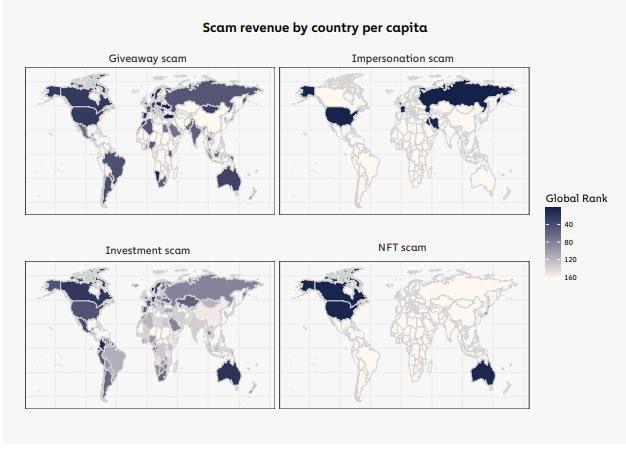
\includegraphics[width=8cm]{scam_2022.png}
    \caption{Scam Revenue by country per capita, Chainalysis Cyber Crime Report 2022}
    \label{fig:my_label}
\end{figure}

\subsection{Hacking}
{\color{blue} Similar to the traditional hacking of computer systems and individual identities, NFTs and NFT accounts can also be hacked by cybercriminals. These attackers target legitimate users and owners of NFTs during the minting or selling phase. \cite{wang2021non} They take advantage of authentication loopholes present in the smart contract to impersonate the user or spoof the owner’s private key to transfer the NFT’s ownership.}

Moreover, the blockchain technology itself and NFT trading platforms like OpenSea have vulnerabilities which hackers can exploit. While the primary components like blockchain and cryptocurrencies are decentralized, the aforementioned NFT platforms actually rely on centralized infrastructures. As a result, it is easier for hackers to invade them using bugs. In fact, a malicious bug infiltrated OpenSea in 2021 which caused 42 NFTs to vanish and caused the platform to lose over 100,000 USD \cite{9755212}. 

\subsection{Phishing Attempts}
Cybercriminals can also execute phishing attacks with NFTs to gain unauthorized access to the funds and assets present in a user’s wallet. The traditional phishing attempts include tricking potential victims into clicking on malicious links and access their sensitive information without their consent. Even though such cybercriminals usually attack organizations such as banks and social media platforms, now they have adopted to the new wave of technologies and invaded the cryptocurrency ecosystems as well. 

These criminals now primarily aim at popular NFT collections by imitating them and tricking the potential buyers into clicking on a fake minting link \cite{roy2023demystifying}. Doing so reveals the sensitive information related to their cryptocurrency wallets and thus the attackers gain access to their wallets. 

\subsection{Rug Pulls}
Rug pull is the term used to represent incidents where a creator sells an NFT or NFT collection at an extremely high price point, only to disappear after making the sale \cite{das2022understanding}. This leaves the investors in deep financial trouble since they end up losing thousands to millions of dollars. The sellers are often influencers in such cases where they have a huge online following, and fans who will trust them and defend them no matter what. 

The influencers advertise these NFT pieces as rare collectibles and promise that these will keep increasing in value in the near future. They convince unsuspecting fans and potential investors that they should start investing as early as possible in order to stay ahead in the game, so that they don’t have to spend too much after the price rises with time. After a few weeks or months, the stock chart actually shows that the price of that NFT has reached almost zero. This causes devastation among the investors who are often regular people with minimal capital in vulnerable states and who need a lot of money in a short span of time.

One such example from the real world is when the rapper Lil Uzi Vert promoted the NFT collection called Eternal Beings to his 8.5 million followers on Twitter in 2021 \cite{rauman2021budding}. After earning from the investments made by his trusting buyers, he ended up deleting all his tweets and the price of the associated NFT tokens took a nosedive. 


\section{Proposed Solutions}
{\color{blue} Since these issues widely vary in nature, attempts to solve them also differ significantly. For instance, one way to detect and prevent wash trading is to use blockchain analysis to analyze the addresses from which the NFTs were sold. This will help us find the correlation between the buying addresses and the selling addresses. If the buying address was funded by the selling address, it can be a potential perpetrator of wash trading.

Another potential solution is to implement self-trade prevention measures which have been already implemented by traditional market exchanges. \cite{victor2021detecting} This mechanism doesn’t allow individual accounts on the publicly traded company IDEX to fill their own orders of buy or sell. 

Know Your Customer (KYC) is another common initiative implemented by such trading companies that compels users to prove their identity with official and verifiable documents. After IDEX adopted this method in 2019, the corresponding wash trading volumes in the centralized system reduced significantly. \cite{victor2021detecting}

For preventing unauthorized access to NFTs and false impersonation of owner accounts, the users should be recommended to choose formal verification while conducting the smart contract and to use cold wallets to keep their private keys secure.}

Such enforced formal verification can also be imposed on users to prevent unauthorized access to NFTs and false impersonation of owner accounts. Doing so while participating in the smart contract and using cold wallets can keep their private keys secure. If the malicious individuals cannot access their private keys, it becomes substantially more difficult for them to spoof the legitimate NFT user's account and assets. As a result, the honest traders  on the platform can increase their assets while the artists can feel motivated to create more of their original pieces.

A contributing factor to the money laundering issues is how most NFT trading platforms only require a connection to a user’s crypto wallet to give him trading permissions \cite{treasurydepartment}. Introducing a mechanism to identify the user’s identity and credentials may reduce the volume of illegitimate money obtained via money laundering with NFTs. Another way to detect it is to put measures in place to automatically identify if the transaction price of an NFT is unusually higher than its market value. 

Certain initiatives have been implemented by researchers to utilize modern scientific approaches for implementing such measures. For instance, Hanna Kim and other Korean researchers came up with DRAINCLoG in 2023 \cite{kim2023drainclog} that can detect accounts which have obtained NFTs illegally using graph neural networks. This model was trained on 83 million NFT transactions executed within 8 months, as well as 742 drainer accounts from 5 sources including Twitter. It has the capacity to take contexts related to NFT transactions and social media to make effective detections.

Another interesting project was implemented by Sayak Saha Roy et. al. in the same year, which trained a machine learning classifier called PhishNFT on over 1,700 URLs to automatically identify NFT phishing scams \cite{roy2023demystifying}. It utilized four ML algorithms including support vector machine, random forest, logistic regression and decision tree.

Ultimately, there needs to be more awareness and spread of knowledge regarding NFt, cryptocurrency and blockchain among the masses. They have the potential to be as crucial as the World Wide Web during the 1990s or the social media during the 2010s. Since they can be an integral part of our daily lives in near future, regular people, especially the younger generations, need to be educated on how the whole ecosystem works. Even if they do not plan to make a career in this path or conduct relevant scientific researches, they still need to know the primary components, features and overall workflow of this system on its surface level. 


\section{Conclusion}
{\color{blue} The whole universe of NFT, cryptocurrency and smart contracts is a relatively novel space for most of us. At the same time, it brings a wide spectrum of exciting opportunities related to art, digital assets and more. Its appeal is growing by the day due to the promises of metaverse where virtual reality and augmented reality will thrive side-by-side. We can then flaunt the NFTs we own to our peers within the metaverse bubble. These digitally unique tokens also enable artists a modern and viable way to earn from their authentic creations.

However, all of these positive scenarios can only become reality when NFT and blockchain technologies implement ethically and legally sound measures to prevent cybercrimes. Taking inspirations from traditional centralized monetary or trading systems and considering novel ideas proposed by experienced in-field researchers, the NFT world can turn into a safe space for both art and trade enthusiasts in near future.}


% include your own bib file like this:
\bibliography{mybib}

\end{document}
